% !TeX root = ../../Thesis.tex
\chapter{Effects of an External Magnetic Field on Stimulated Raman Scattering}
\label{chp:magSRS}

\section{Motivation}

Suppress SRS to reduce harmful electrons and reflectivity, or enhance if it actually makes good electrons (in the case of shock-ignition).

\section{How does magnetic suppression work?}

Start by replicating results from \cite{Winjum2018}

\begin{figure}
    \centering
    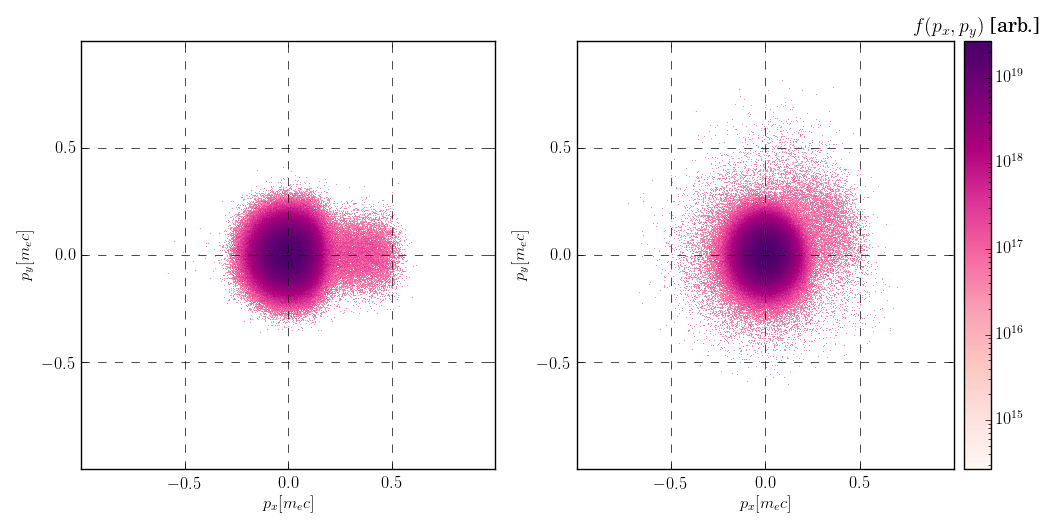
\includegraphics[width=0.99\textwidth]{Chapters/C5_magSRS/best_px_py_compare.png}
    \caption{Caption}
    \label{fig:my_label}
\end{figure}{}